% 2015陕西文 q20 图1：椭圆 x^2/2+y^2=1，过(1,1)斜率为k的动直线(取k=0.8)交椭圆于P,Q，A(0,-1)
\usetikzlibrary{arrows.meta}
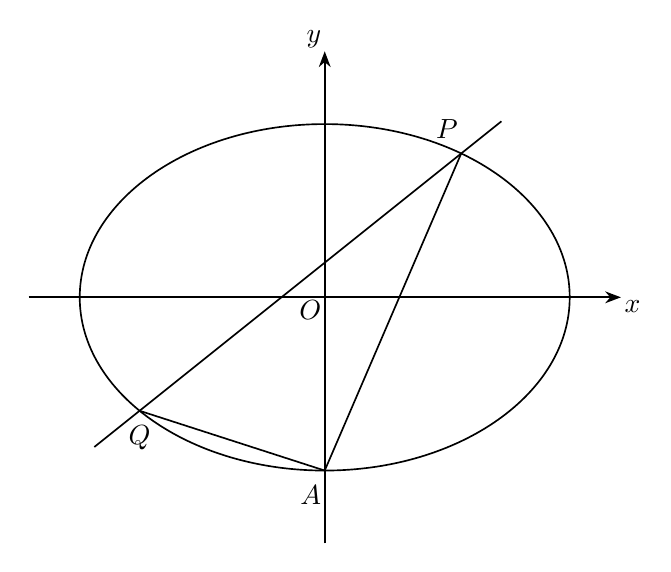
\begin{tikzpicture}[x=2.2cm,y=2.2cm,line width=.6pt,font=\normalsize,>=Stealth]
  \draw[->] (-1.71,0) -- (1.71,0) node[below right,inner sep=1pt] {$x$};
  \draw[->] (0,-1.42) -- (0,1.42) node[above left,inner sep=1pt] {$y$};
  \draw (0,0) ellipse [x radius=1.41421,y radius=1];
  \draw (-1.33000,-0.86400) -- (1.02000,1.01600);
  \draw (0.78798,0.83039) -- (0,-1);
  \draw (-1.06868,-0.65495) -- (0,-1);
  \node[below left,inner sep=1pt] at (0,0) {$O$};
  \node[below left,inner sep=1pt,yshift=-4pt] at (0,-1) {$A$};
  \node[above left,inner sep=1pt,yshift=4pt] at (0.78798,0.83039) {$P$};
  \node[below,inner sep=1pt,yshift=-4pt] at (-1.06868,-0.65495) {$Q$};
\end{tikzpicture}
